\documentclass{article}

% if you need to pass options to natbib, use, e.g.:
% \PassOptionsToPackage{numbers, compress}{natbib}
% before loading nips_2016
%
% to avoid loading the natbib package, add option nonatbib:
% \usepackage[nonatbib]{nips_2016}

\usepackage[final]{nips_2016}

% to compile a camera-ready version, add the [final] option, e.g.:
% \usepackage[final]{nips_2016}

\usepackage[utf8]{inputenc} % allow utf-8 input
\usepackage[T1]{fontenc}    % use 8-bit T1 fonts
\usepackage{hyperref}       % hyperlinks
\usepackage{url}            % simple URL typesetting
\usepackage{booktabs}       % professional-quality tables
\usepackage{amsfonts}       % blackboard math symbols
\usepackage{nicefrac}       % compact symbols for 1/2, etc.
\usepackage{microtype}      % microtypography
\usepackage{graphicx}
\usepackage{cite}

\title{Neural Networks for Learning Stock Market Features}

\author{
  Dan Schmidt \\
  Department of Mathematics\\
  Harvey Mudd College\\
  Claremont, CA 91711 \\
  \texttt{dschmidt@hmc.edu} \\
}

\begin{document}

\maketitle

\begin{abstract}
    Predicting stock market prices from observed data is a highly challenging
    but potentially lucrative task. The usual procedure for finding
    profitable patterns is to have a hypothesis about how the market works,
    and then to engineer features that model this hypothesis. In this paper,
    I investigate potential methods for exctracting potential features from
    stock price and volume data. First, both linear (PCA) and non-linear
    (autoencoder) dimensionality techniques are applied to windowed data.
    Then a layered supervised network is trained against future returns 
    to try to find features that correspond to predictive power. In each
    case, a GPU is used to train millions of data points effectively. I
    find that the supervised neural network trained on price and volume
    data could be used for what is in theory a profitible trading strategy. 
\end{abstract}

\section{Introduction}

The hot machine learning topic of the moment is so called deep-learning. The
idea with deep learning is not to improve models by hand-engineering features
but by turning loose a large amount of computational power on neural networks
with many hidden layers. The idea is that the layers learn a hierarchy of 
features that have large predictive power for the goal the network is trained
against. My approach here is not to use the most cutting-edge or trendy
deep learning techniques but to use a deep learning software system, Keras 
with a Theano back end, to try basic feature learning on stock market data. 

Neural networks are some of the most powerful learning algorithms known due
to their non-linear nature and ability to learn any continuous function.
For complciated non-linear regression problems, neural networks serve
as a highly efficient function basis.
The challenges of using neural networks are that they are difficult to
interpret, resistant to simple probabilistic interpretation, and difficult
to train without overfitting. These downsides can be mitigated by feeding
them a lot of data. To do this, one needs both an abundance of data and
a computing system capable of processing that much data in reasonable time
frames. For my data, I use a couple years worth of minute-resolution stock
price and volume data provided by PiTrading.com. For my efficient computation
system, I train my networks on a GTX 750ti, a GPU that is a couple of years old
but still is orders of magnitude faster to perform the matrix operations than 
my CPU.

\section{The Problem}


Much research has been done to address the question of predicting future prices
just from looking at the stock's data. The efficient market hypothesis is the
economic theory that any predictive power in the markets is almost 
instantaneously arbitraged away, so that without outside information, stock prices 
follow random walks (citation). The controversial field of technical analysis holds the
opposite theory, that there are predictive patterns in stock price movements.

\section{The Data}

\subsection{Format and Preprocessing}
The data is minute-resolution price and volume data on SP500 stock tickers and 
a few hundred major ETFs.
The data is provided in CSV format from PiTrading. This raw data is then processed
out of CSV files into Python pandas dataframes, which are saved in a binary format
to disk for faster processing later. 

A major note is that there are many missing price dates, and that the data also may
contain survivor bias. These issues are mitigated in this analysis by selecting
tickers and time frames that have mostly ($95\%$) data and using only relatively
short time frames over which established companies are trading in a normal environment.

\subsection{Returns: Working in Percent Return Space}

One important starting point for analyzing price data is to work in return space.
This is because the raw dollar value of a stock doesn't really mean anything. The
data used in this paper does not have market cap information, and so the prices
cannot be weighted that way. That leaves three options:

\begin{enumerate}
    \item
        Return space, i.e.
        \[ r_t = \frac{X_t - X_{t-1}}{X_{t-1}} \]
    \item
        Log return space, i.e.
        \[ l_t = \log\left( 1+ r_t \right) = \log\left( \frac{X_t}{X_{t-1}} \right) = \log(X_t) - \log(X_{t-1}) \] 
    \item
        Normalized returns
        \[ r_{t} = \frac{1}{\hat{\sigma}(X)} \frac{X_t - X_{t-1}}{X_{t-1}} \]
        where we divide by the estimated standard deviation.
\end{enumerate}

Return space is convenient in that the results are easily interpretible, as in they are
just fractional movements in price. The reasons to prefer log return space are that
often returns are not normally distributed, but the log of the returns is, and that
log returns have nice computational properties where you can accumulate with sums
rather than cumulative products. Normalized returns are mostly useful for doing
market basket analysis, as some stocks may have more volatility than others. 

\section{Linear Dimensionality Reduction: PCA}

An initial idea for improving model performance would be to reduce the dimensionality
of the data before the model is fit. One way to do this would be to 
see if windowed hours can be projected onto a linear subspace.
We try a PCA analysis on sliding window price data to see if this
has any viability as a dimensionality reduction strategy. The results are shown
in figure \ref{fig:pca}. 

\begin{figure}[h]
    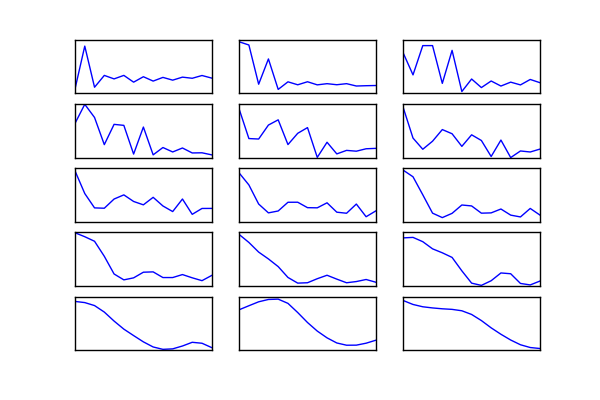
\includegraphics[width=0.5\textwidth]{pca_features}
    \caption{The eigenvectors of PCA.}
    \label{fig:pca}
\end{figure}

It turns out this projection is not
very useful here. First, the eigenvector corresponding to the
principal component is not qualitatively distinguishable from
the component that explains the least variance. Second, the
decay in the eigenvalues is much slower than what we would
expect if PCA discovered underlying linear structure. Part of
the problem with this analysis is that for a windowed time series,
one would expect that features should be somewhat invariant in
time. Thus any structure found here would have to persist in sliding
through the windows, which it looks like is not the case. We need
a model that has more knowledge of the structure of the data. 


\section{Non-linear: Neural Nets}

Another way to reduce the dimensionality for prediction is to let the
neural network learn features itself by stacking hidden layers into the network.
This is the approach used here. 

\subsection{Unsupervised Approach: Autoencoder}

Although PCA did not seem to recover any underlying structure in the 
data, it is possible that there is some non-linear relationships within
the data. The technique tried here for to find this structure is to
train an autoencoder, a neural network that learns the identity function.
The idea of an autoencoder is that there are at least two non-linear layers
between the input vector and the output vector. The first layer maps the
input vector to some lower dimensional subspace. This lower dimensional
subspace hopefully is a more meaningful representation of the data, and
can be used to find interesting non-linear patterns. 

\begin{figure}[h]
    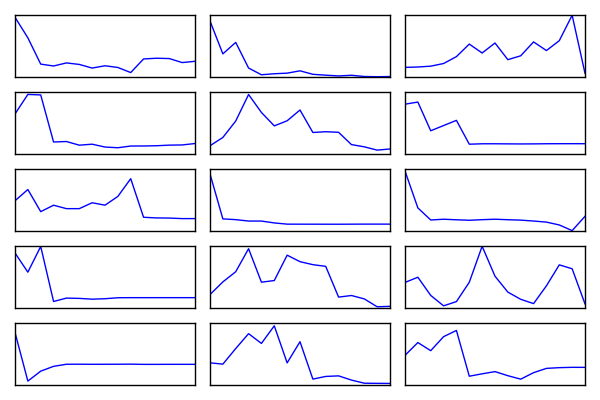
\includegraphics[width=0.5\textwidth]{autoencoder_features}
    \caption{Extracted 15-minute window representations from a a year with of
    minute price movements on AAPL. These features are the weights on the first layer
    of a four-layer network, accumulated so that they represent stock-chart price
    movements.}
    \label{fig:autoencoder_features}
\end{figure}

\begin{figure}[h]
    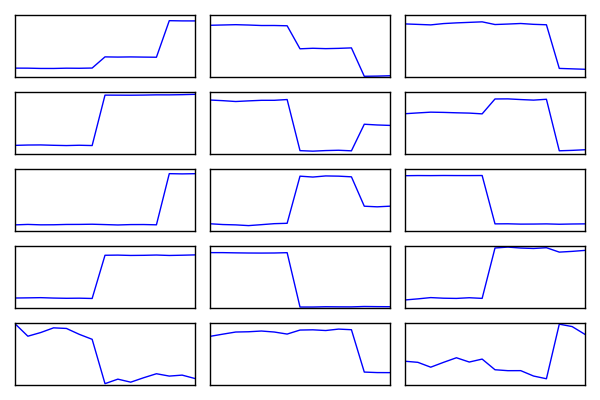
\includegraphics[width=0.5\textwidth]{sparse_features}
    \caption{Same network trained on the same data as \ref{fig:autoencoder_features},
    except now $l1$ regularized to enforce sparsity. Note the more jagged learned
    features, as flat lines are due to the sparse feature construction}
    \label{fig:sparse_features}
\end{figure}

\subsection{Supervised Approach: Windowed Multi-Layer Perceptron}

There are various network architectures one could use to predict time
series with neural networks. The model here is a standard multi-layer
perceptron as described in Bishop \cite{bishop1995neural}.

\begin{figure}[h]
    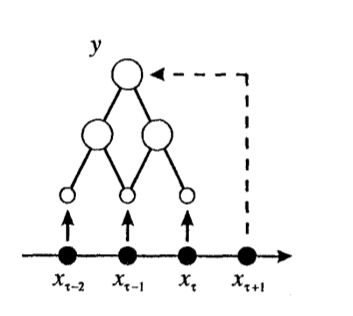
\includegraphics[width=0.5\textwidth]{bishop_ts_nn}
    \caption{Diagram of the windowed network to predict one step forward in the
    time series.}
    \label{fig:mlp_ts}
\end{figure}

As shown in figure \ref{mlp_ts}, the idea is that the time series is windowed
into sections. These sections are then used as features for predicting the next
element in the time series. The layers stacked in between are nonlinear
combinations designed to learn latent features in the data that predict the
outcome. The network is trained by sliding a window over a long period of stock
data and minimizing the error in predicting one time step forward.

With the autoencoder, the network was set to learn a set of non-linear features
that best could replicate any window of returns. By training the network 
against future returns, we look more for price (and volume)
features that best predict forward returns. This more difficult training
objective may find different features than an autoencoder. 

The learned features on the same data set as PCA and the autoencoder is shown in
figure \ref{fig:mlp_feats}.

\begin{figure}[h]
    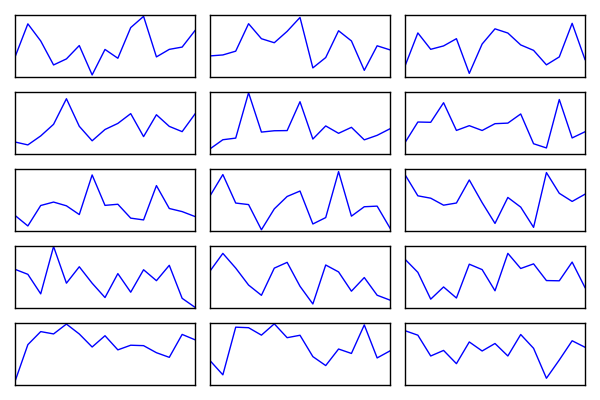
\includegraphics[width=0.5\textwidth]{mlp_feats}
    \caption{Features learned in the supervised network}
    \label{fig:mlp_feats}
\end{figure}

\section{Bayesian Analysis of The Network}

Bayesian methods can be very helpful in training and analyzing
neural networks. One of my goals for this project was to use
these Bayesian methods to help train better networks. Unfortunately,
the hyperparameter estimation worked better by hand and I was unable
to effectively compute the Hessian of my network as is needed by the
method to analyze error in predictions. But here I lay out the
theoretical basis for how Bayesian techniques can be useful for
neural network training and evaluation. These are mostly learned
from the logistic regression example in class and Bishop \cite{bishop1995neural}.

Assume our model has weights $w$ and hyperparameters $\gamma$. Our task
is to learn an approriate function $p(y|x, w, \gamma)$, so we seek to
optimize
\[ argmax_{w, \gamma} p(w, \gamma |D) \]
The frequentist approach to fitting this function is to choose a set
of possible hyperparameters and search through this parameter space
optimizing the weights each time. The results are then checked on
a validation set, and the optimal combination of parameters are chosen
this way. The problem with this approach is that for neural networks,
the hyperparameter space can be huge and so difficult
to effectively search. In addition, unless one has a lot of data, it is
difficult to not overfit either the training set or validation set. Finally,
once one has a model, it is difficult to a sense of what the error bars should
be on the models predictions. Approaching this problem with a Bayesian 
perspective provides some ways to get around these problems.\\ \\

The first step to using Bayesian techniques on neural networks is to choose
a prior on the weights. Here for simplicity we use a Gaussian model

\[ p(w) = \frac{1}{Z_W(\alpha)} \exp \left( -\frac{\alpha}{2} ||w||^2  \right) \]
where $\alpha$ is a hyperparameter and $Z$ is just a normalization constant.
Another choice to make is the distribution of error. Here again we use a
Gaussian model,

\[ p(y| x, w) \propto \exp\left( -\frac{\beta}{2} (f(x,w)-y)^2 \right) \]

\subsection{Evaluating Error Bars}

Assume we have optimal choices for our hyperparameters. We can
use the distributions we have estimated so far to get an expression
for error bars on the output of our regression. To do so, we wish
to compute the integral 

\[ p(y|x, D) = \int p(y|x,w) p(w|D)  dw \]

$p(y|x, w)$ is our model for distribution of noise, and $p(w|D)$ is
the model for the weights given the data. The approximation we use
is the same approximation given in section $8.4$ of Murphy \cite{murphy2012machine}.
We approximate this integral with a linear expansion around $f(x; w_{MAP})$.
If 
\[ g = \nabla_w y|_{w_{MAP}} \]
and if $H$ is the Hessian matrix, then 
\[ p(y|x, D) = \frac{1}{2\pi \sigma_t^2} \exp\left(-\frac{(y-f(x;w_{MAP}}{2\sigma_t^2} \right) \]
where
\[ \sigma_t = \frac{1}{\beta} + g^T H^{-1} g \]

This $\sigma_t$ is our error bar, and evaluating it mostly involves evaluating the
Hessian matrix $H$ at a given point. The first term is a standard noise term
from our model of the noise on our data. Either term can dominate depending
on the Hessian matrix.

\section{Implementation and Results}

\subsection{Implementation}
The model was implemented using the standard Python SciPy stack. For
the neural network model, the Keras library with a Theano backend was
used. This let me train my models on my GPU, which gave higher
performance training for faster iteration on trying different models.

\subsection{Results}
The supervised version of the nerual network showed the most promise for
being the basis of a trading strategy. The network was trained on
the $30$ symbols in the Dow Jones Industrial average over a period of
two years, representing approximately $1.2$ million data points. This
was done in two ways: first, a network was trained on each symbol. These
networks try to learn features unique to each symbol. 
The predictions from these networks were then used as a trading strategy. The trading
strategy is to buy if the predicted future movement is up more than one standard
deviation, and to sell if the prediction is down more than one standard deviation.
The results from these models are shown in table \ref{profit_table}. Without
including fees or execution difficulties in buying and selling at the minute
time scale, this strategy appears to be profitable for 24 of 30 symbols in the
Dow Jones Industrial Average, trained on 2013 and tested on 2014.

\begin{tabular}{lll}
    Symbol & Profit (annualized return) & Sharpe Ratio \\ 
\toprule

    AAPL & 0.16 & 0.37 \\
    AXP & 1.30 & 3.13 \\
    BA & 1.16 & 1.88 \\
    CAT & 5.73 & 10.10 \\
    CSCO & -0.97 & -3.11 \\
    CVX & 0.58 & 2.07 \\
    DD & 0.43 & 1.19 \\
    DIS & -0.16 & -0.42 \\
    GE & 1.49 & 4.77 \\
    GS & -2.26 & -6.06 \\
    HD & 2.01 & 5.94 \\
    IBM & 0.68 & 2.05 \\
    INTC & -3.07 & -8.21 \\
    JNJ & 0.67 & 2.03 \\
    JPM & 0.35 & 0.91 \\
    KO & 0.34 & 1.06 \\
    MCD & -0.88 & -2.65 \\
    MMM & 3.63 & 10.99 \\
    MRK & 3.22 & 7.35 \\
    MSFT & 0.65 & 1.55 \\
    NKE & 2.08 & 6.04 \\
    PFE & 2.92 & 7.19 \\
    PG & 1.57 & 4.61 \\
    TRV & 0.36 & 1.39 \\
    UNH & 2.86 & 6.65 \\
    UTX & 1.99 & 4.59 \\
    V & 4.83 & 9.29 \\
    VZ & -1.32 & -3.22 \\
    WMT & 2.21 & 7.10 \\
    XOM & 1.16 & 3.73 \\
\end{tabular}

Another network was constructed that was trained on all $1.2$ million data points
to see if the large amount of data would reveal any interesting overall stock
market patterns. The features learned are shown in \ref{fig:big_feats}.

\begin{figure}[h]
    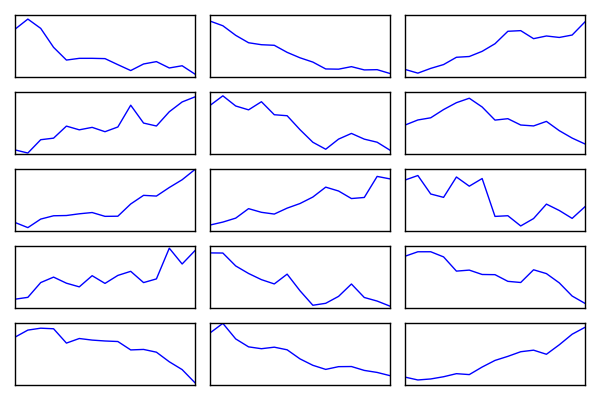
\includegraphics[width=0.5\textwidth]{mlp_feats_big}
    \caption{Features learned by training on millions of data points across symbols.}
    \label{fig:big_feats}
\end{figure}


\section{Conclusions}

In conclusion, on the level of minute data there do seem to be exploitable patterns
in stock price data. While linear methods struggle, non-linear neural networks
find subtle structure. This analysis is very cursory 

\bibliography{citations}{}
\bibliographystyle{plain}

\nocite{*}

\end{document}
